\documentclass{article}

\usepackage{graphicx}
\usepackage{tikz}
\usepackage{tikzsymbols}
\usetikzlibrary{calc,patterns,shapes.geometric}
\pagestyle{empty}
\usepackage[margin=0pt]{geometry}
\geometry{papersize={14in,12in}}

\def\centerarc[#1](#2)(#3:#4:#5){\draw[#1] ($(#2)+({#5*cos(#3)},{#5*sin(#3)})$) arc (#3:#4:#5);}

\begin{document}
	\begin{figure}
		\centering
		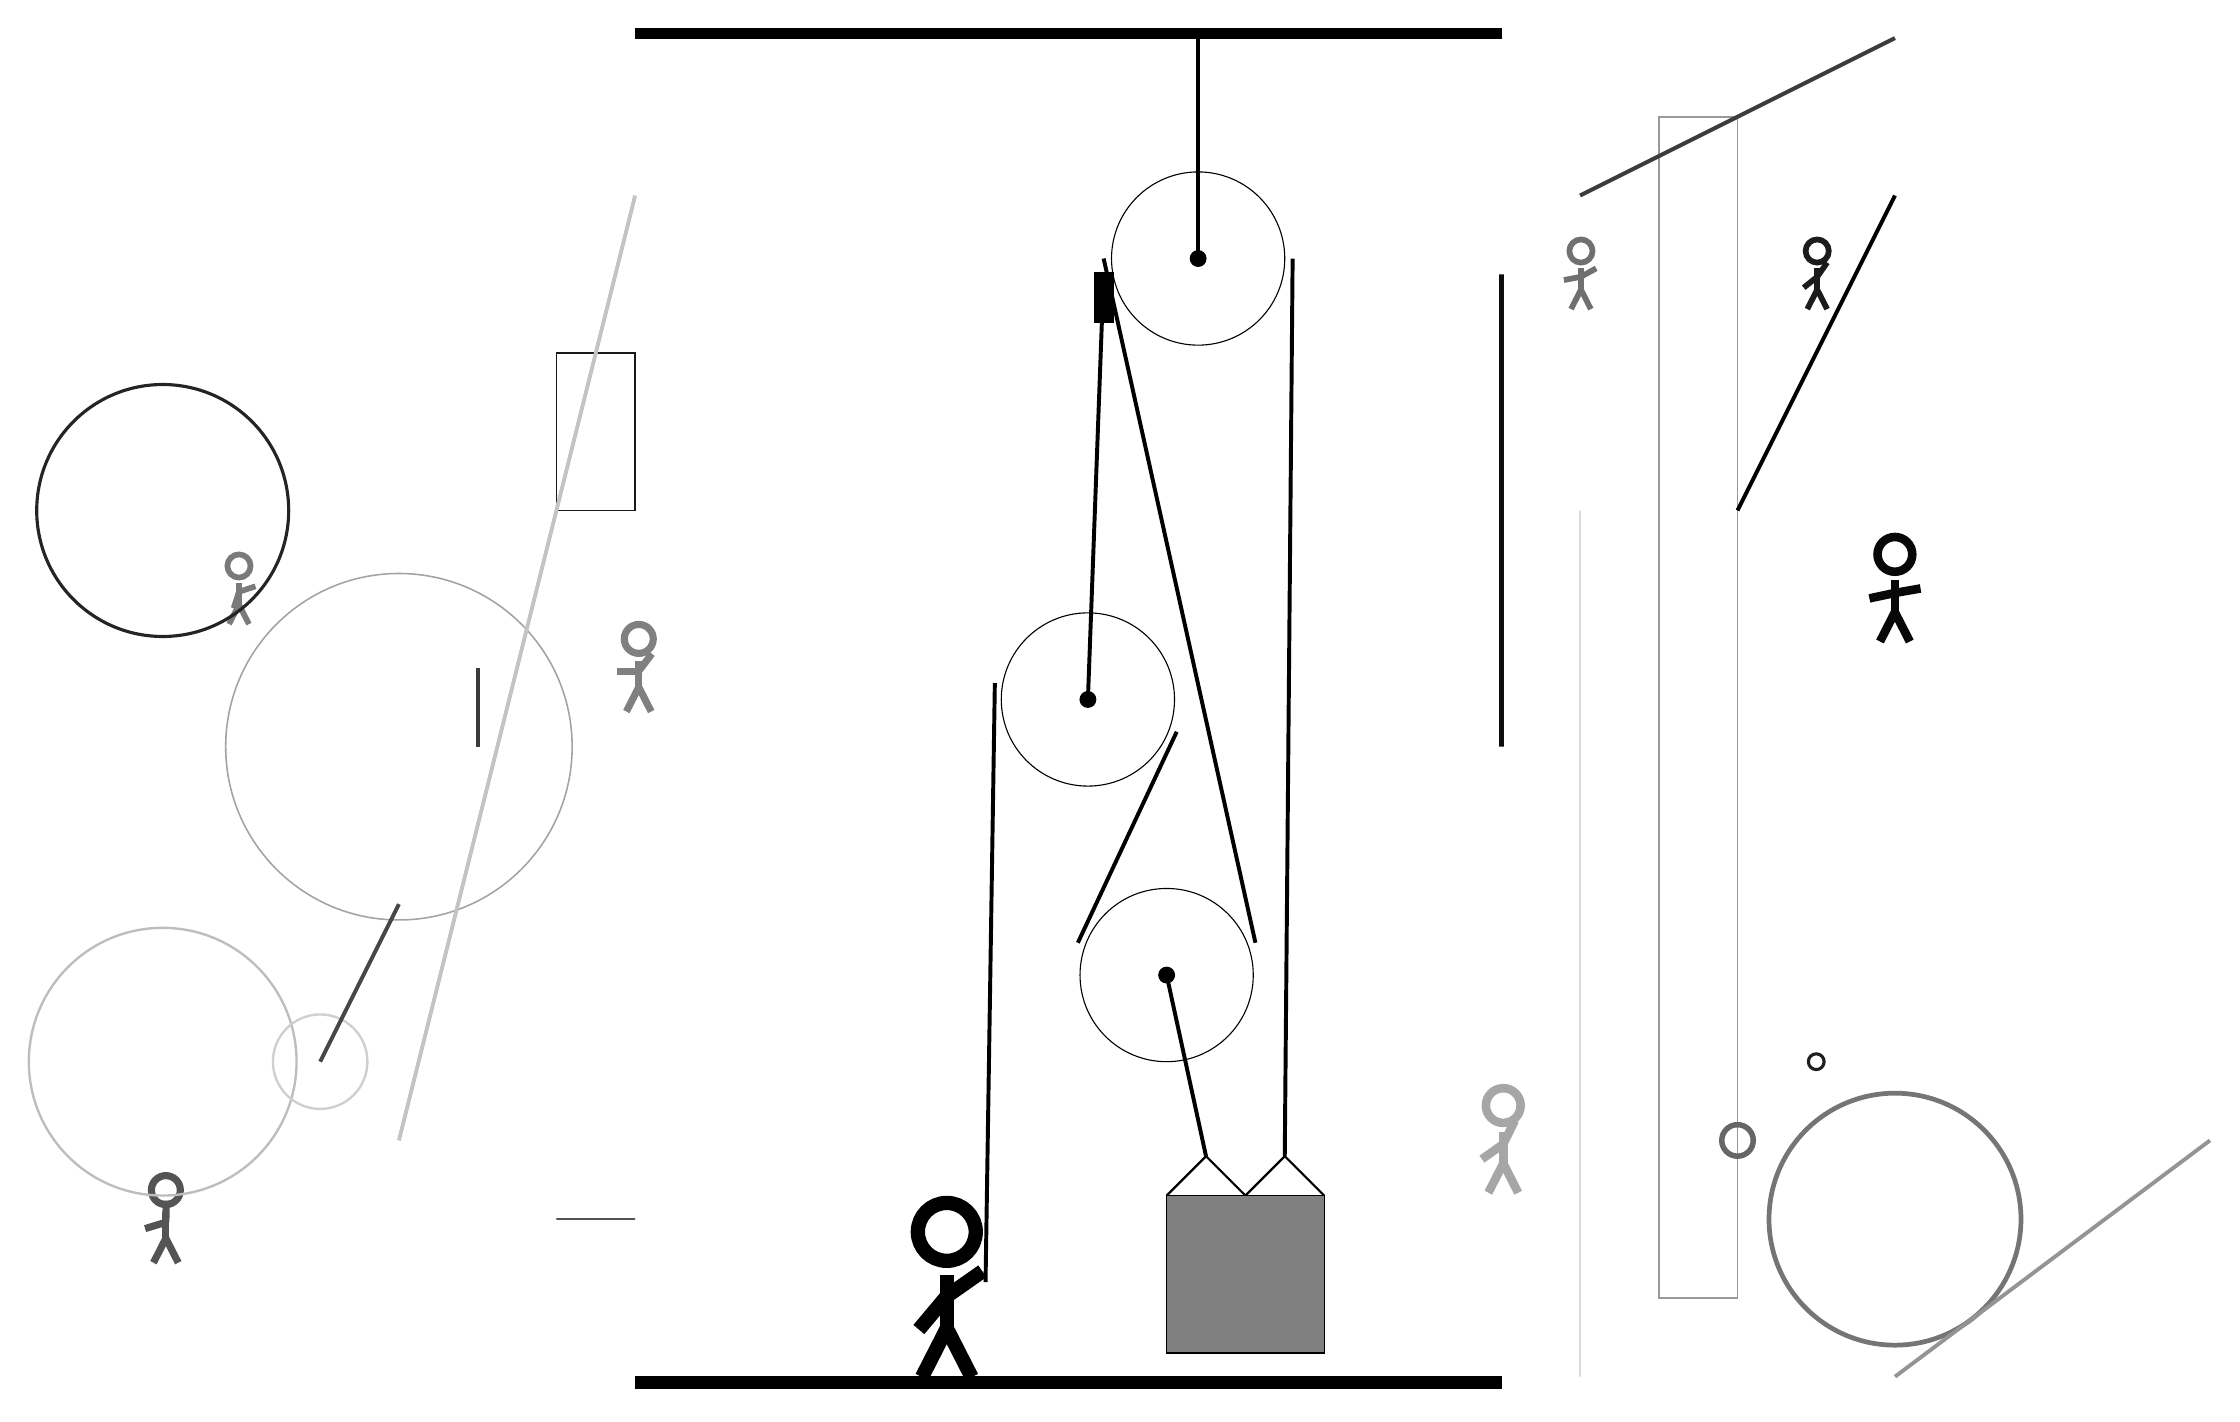
\begin{tikzpicture}
			%%%%% START %%%%%
			
			\draw[fill=black] (-6, 14) rectangle (5, 14.125);
			
			\draw (-0.25, 5.6) circle (1.1);
			\draw[fill=black] (-0.25, 5.6) circle (0.1);
			
			\draw [line width=0.2mm, color=black!36](-9, 5) circle (2.2);
			
			\draw[line width=0.2mm, color=black!68] (-7, -1) rectangle (-6, -1);
			\node[line width=0.6mm, color=black!35] at (5, 0) {\Strichmaxerl[6][35][64]};
			\node[line width=0.6mm, color=black!50] at (-6, 6) {\Strichmaxerl[5][0][53]};
			\draw [line width=0.4mm, color=black!88](9, 1) circle (0.1);
			\node[line width=0.2mm, color=black!67] at (-12, -1) {\Strichmaxerl[5][17][89]};
			\draw[line width=0.7mm, color=black!95] (5, 5) rectangle (5, 11);
			
			\draw[line width=0.2mm, color=black!40] (7, 13) rectangle (8, -2);
			\draw [line width=0.3mm, color=black!26](-12, 1) circle (1.7);
			\draw [line width=0.7mm, color=black!60](8, 0) circle (0.2);
			
			\node[line width=0.6mm, color=black!52] at (-11, 7) {\Strichmaxerl[4][72][18]};
			\draw [line width=0.4mm, color=black!86](-12, 8) circle (1.6);
			\draw [line width=0.3mm, color=black!19](-10, 1) circle (0.6);
			\node[line width=0.3mm, color=black!97] at (10, 7) {\Strichmaxerl[6][12][10]};
			\node[line width=0.3mm, color=black!89] at (9, 11) {\Strichmaxerl[4][39][55]};
			\draw[line width=0.2mm, color=black!90] (-6, 10) rectangle (-7, 8);
			
			\draw[line width=0.5mm, color=black!23](-9, 0) -- (-6, 12);
			\draw[line width=0.5mm, color=black!77](-8, 6) -- (-8, 5);
			\draw [line width=0.6mm, color=black!54](10, -1) circle (1.6);
			
			\draw[line width=0.5mm, color=black!76](6, 12) -- (10, 14);
			\draw[line width=0.5mm, color=black!42](10, -3) -- (14, 0);
			
			\node[line width=0.5mm, color=black!56] at (6, 11) {\Strichmaxerl[4][11][29]};
			
			\draw[line width=0.5mm, color=black!100](10, 12) -- (8, 8);
			\draw[line width=0.3mm, color=black!15] (6, -3) rectangle (6, 8);
			\draw[line width=0.5mm, color=black!72](-10, 1) -- (-9, 3);
			
			
			\draw (0.75, 2.1) circle (1.1);
			\draw[fill=black] (0.75, 2.1) circle (0.1);
			
			\draw (1.15, 11.2) circle (1.1);
			\draw[fill=black] (1.15, 11.2) circle (0.1);
			\draw[very thick] (1.15, 11.2) -- (1.15, 14);
			
			\draw[thick]  (0.75, -0.7) -- (1.25, -0.2) -- (1.75, -0.7) -- (2.25, -0.2) -- (2.75, -0.7);
			\draw[fill=black!50] (0.75, -0.7) rectangle (2.75, -2.7);
			
			\draw[line width=0.5mm] (-0.25, 5.6) -- (-0.05, 11.0);
			\draw[line width=0.5mm, fill=black](-0.15, 10.4) rectangle (0.05, 11.0);
			\draw[line width=0.5mm] (-1.55, -1.8) -- (-1.4318, 5.8083);
			\centerarc[line width=0.5mm](-0.25, 5.6)(-20:170:1.2000000000000002);
			\draw[line width=0.5mm] (0.8776, 5.1896) -- (-0.3776, 2.5104);
			\centerarc[line width=0.5mm](0.75, 2.1)(160:380:1.2000000000000002);
			\draw[line width=0.5mm] (1.8776, 2.5104) -- (-0.05, 11.2);
			\draw[line width=0.5mm](0.75, 2.1) -- (1.25, -0.2);
			\centerarc[line width=0.5mm](1.15, 11.2)(0:180:1.2000000000000002);
			\draw[line width=0.5mm] (2.35, 11.2) -- (2.25, -0.2);
			
			\node at (-2, -1.9) {\Strichmaxerl[10][50][35]};
			
			\draw[fill=black] (-6, -3) rectangle (5, -3.15);
			
			%%%%% END %%%%%
		\end{tikzpicture}
	\end{figure}	
\end{document}